\documentclass[10pt]{article}

% ── Packages ─────────────────────────────────────────────────────────────────
\usepackage[margin=1.2in,top=1in,bottom=1.1in]{geometry}
\usepackage{amsmath,amssymb,amsthm}
\theoremstyle{plain}
\newtheorem{theorem}{Theorem}[section]
\newtheorem{proposition}[theorem]{Proposition}
\newtheorem{corollary}[theorem]{Corollary}
\newtheorem{lemma}[theorem]{Lemma}
\theoremstyle{definition}
\newtheorem{definition}[theorem]{Definition}
\newtheorem{remark}[theorem]{Remark}
\usepackage{graphicx}
\usepackage{booktabs}
\usepackage{colortbl,xcolor}
\usepackage[hidelinks]{hyperref}
\usepackage{subcaption}
\usepackage{placeins}
\usepackage{tikz}
\usetikzlibrary{arrows.meta,shapes.geometric,positioning,fit,
                calc,decorations.pathreplacing,patterns,backgrounds}
\usepackage{algorithm}
\usepackage{algpseudocode}

\usepackage{cite}
\usepackage{enumitem}
\setlist{noitemsep,topsep=2pt}

\definecolor{ours}{RGB}{220,235,255}

%── DeepMind palette (Figure 2) ──────────────────────────────────────────────
\definecolor{dmBlue}{HTML}{1A73E8}
\definecolor{dmBlueL}{HTML}{E8F0FE}
\definecolor{dmTeal}{HTML}{00897B}
\definecolor{dmTealL}{HTML}{E0F2F1}
\definecolor{dmGreen}{HTML}{34A853}
\definecolor{dmGreenL}{HTML}{E6F4EA}
\definecolor{dmAmber}{HTML}{E37400}
\definecolor{dmAmberL}{HTML}{FEF3CD}
\definecolor{dmGray}{HTML}{5F6368}
\definecolor{dmGrayL}{HTML}{F1F3F4}
\definecolor{dmGrayM}{HTML}{DADCE0}
\definecolor{dmText}{HTML}{202124}
% ── Title ─────────────────────────────────────────────────────────────────────
\title{\textbf{Structure-Based UAV Visual Geo-Localization via\\
Delaunay Triangulation and Ekeland Free-Cone Angle Descriptors}}

\author{%
  Author One$^{1}$ \quad Author Two$^{1}$ \quad Author Three$^{1}$\\[4pt]
  $^{1}$Institute of Mathematical and Computational Sciences (IMACS), \\
  Ho Chi Minh City University of Technology (HCMUT), \\
  268 Ly Thuong Kiet Street, District 10, Ho Chi Minh City, Vietnam. \\[2pt]
  \texttt{\{author1,author2,author3\}@hcmut.edu.vn}
}
\date{}

\begin{document}
\maketitle

% ─────────────────────────────────────────────────────────────────────────────
\begin{abstract}
Accurate geo-localization of unmanned aerial vehicles (UAVs) in GPS-denied
environments remains a core challenge for autonomous navigation.
We propose a scene-agnostic absolute visual localization framework that
identifies the UAV's 2-D geographic position by matching a single nadir image
against a geo-referenced satellite map using purely geometric building
footprint descriptors, requiring no scene-specific training.
Buildings are segmented by a pre-trained Mask R-CNN; each polygon is
decomposed into triangles by Constrained Delaunay Triangulation (CDT), and
each triangle is encoded with a 5-dimensional descriptor
$f = (\alpha_1,\alpha_2,e_1,e_2,e_3)$ comprising two sorted interior angles
and three \textbf{Maximal Free Cone Angles (MFCA)}---a geometric quantity
measuring the largest obstacle-free angular sector at each vertex.
The MFCA is directly inspired by Ekeland's variational principle (1974):
the principle guarantees a critical point where no improvement is achievable
without a proportional distance cost; we instantiate this as a
\emph{kernel expansion} $P_{\mathrm{sub}}$---the largest polygon formed by
merging adjacent CDT triangles such that all three original triangle vertices
remain on the boundary of the result.
This stopping criterion is the direct geometric analogue of Ekeland's
cone-criticality condition: the polygon cannot be expanded further while
keeping the triangle vertices as boundary (critical) points.
The Ekeland angle $e_v$ at each vertex is then the exterior angle of
$P_{\mathrm{sub}}$ at $v$, computed in $O(1)$ per vertex by an
edge-anchored half-plane construction with no sweep required.
Satellite patch descriptors are indexed offline in a KD-tree ($\ell_1$ metric);
online matching runs in $O(M\log N)$ time per query.
Quantitative evaluation on the UAV-VisLoc benchmark, ablation study, season
and altitude stratifications, and sensitivity analyses are to be reported
(TBR) upon completion of full experiments.
\end{abstract}

% ─────────────────────────────────────────────────────────────────────────────
\section{Introduction}
\label{sec:intro}

UAVs depend on GNSS for position fixes in nearly every operational domain:
search-and-rescue, precision agriculture, infrastructure inspection, and
military reconnaissance.
Yet GNSS is unavailable in urban canyons, jammed in contested airspace, and
unreliable indoors---scenarios that are precisely those requiring the most
reliable autonomy.
A single GNSS outage during a search-and-rescue operation can redirect a UAV
kilometres from the target zone.
In contested airspace, GPS jamming has been documented to deny localization
entirely for extended periods~\cite{murrian2021gnss,dovis2015gnss}.
For emergency responders, infrastructure inspectors, and autonomous delivery
operators, GNSS failure is not a theoretical edge case---it is the operational
norm in precisely the environments these platforms are deployed.
Vision-based absolute visual localization (AVL) addresses this gap by
recovering the UAV's 2-D geographic position from onboard camera images matched
against a pre-stored reference map, with no satellite signal
required~\cite{couturier2021review,ouyang2024cfbvm}.

The dominant difficulty in UAV-to-satellite AVL is the \emph{cross-view
appearance gap}: satellite maps are orthorectified nadir projections captured
in a fixed season, while UAV images arrive at varying altitude, heading, roll,
pitch, time of day, and season.
Existing methods expose a fundamental trilemma:
(i)~\emph{Appearance-based methods} (SIFT, ORB, deep cross-view
networks~\cite{goforth2019gps,fan2024sspt}) rely on pixel-level signals that
change across season, altitude, and lighting---SIFT achieves zero Recall@10 on
MAFS-10 after 1,630\,s of computation~\cite{yuan2025swapf},
confirming that texture descriptors cannot bridge the nadir gap.
(ii)~\emph{Deep learning methods} overcome the appearance gap by learning
invariant embeddings, but require scene-specific retraining, making them
impossible to deploy on a new city map within hours.
(iii)~\emph{Vector map methods} exploit shape rather than texture, but existing
approaches (BRM~\cite{choi2020brm}, CFBVM~\cite{ouyang2024cfbvm}) operate on
whole-building statistics and lose the \emph{spatial context between buildings},
making them poorly discriminative in dense urban blocks where many buildings
share similar individual shapes.
No existing training-free method simultaneously encodes both intra-building
shape and inter-building spatial context within a single descriptor.

Our key insight is that \emph{building footprint geometry} is stable across
all of these appearance variations: a polygon extracted from a nadir UAV image
and the same polygon in a satellite map agree in shape regardless of altitude,
season, or illumination.
We exploit this by (i)~decomposing each building polygon into triangles via CDT
and (ii)~encoding each triangle with a 5-D descriptor of pure angular
quantities invariant to scale, rotation, and appearance.
The free-space component of this descriptor---the Maximal Free Cone Angle
(MFCA)---is directly inspired by Ekeland's variational principle~\cite{ekeland1974}:
the principle characterises a point of maximal local stability as the apex
of the largest cone that touches but does not cross a function's graph;
we instantiate this cone not over a function graph but over a 2-D polygon
boundary, yielding a scalar that encodes \emph{how much local geometric
freedom exists at each building vertex}.

The ability to localize a UAV without GPS, without scene-specific training,
and with only a pre-stored satellite map represents a step toward truly
\emph{map-portable autonomy}: a platform pre-loaded with satellite imagery of
any new city can begin operating immediately upon arrival, with no training
phase required.
This capability has direct implications for rapid disaster response, military
forward deployment, and commercial UAV scalability where per-scene model
training is operationally infeasible.

\paragraph{Contributions.}
\begin{enumerate}
\item \textbf{Edge-anchored Ekeland angle (MFCA).}
      We derive the Ekeland angle $e_v$ from first principles via a two-phase
      construction: (i)~expand the kernel triangle into a maximal polygon
      $P_{\mathrm{sub}}$ whose stopping condition directly instantiates
      Ekeland's cone-criticality---merging halts precisely when any of the
      three original triangle vertices would leave the boundary; (ii)~compute
      $e_v$ as the exterior angle of $P_{\mathrm{sub}}$ at $v$ via an
      edge-anchored half-plane selection (Section~\ref{sec:mfca}).
      The result is \emph{exact} (no quantization), $O(1)$ per vertex, and
      rigorously grounded: the kept sector's bounding ray is tangent to the
      polygon boundary---the literal ``cone touches but does not cross''
      condition of Ekeland's principle.
\item \textbf{5-D geometric feature}
      $f = (\alpha_1,\alpha_2,e_1,e_2,e_3)$ combining two sorted interior
      angles and three independently sorted MFCAs, providing complementary
      shape and free-space context (Section~\ref{sec:feat}).
\item \textbf{Scalable offline index.}
      Satellite patch descriptors are indexed in a KD-tree with $\ell_1$ metric,
      reducing online position matching from $O(MN)$ to $O(M\log N)$
      (Section~\ref{sec:kdtree}).
\item \textbf{Plurality-vote position estimator.}
      UAV triangle votes aggregate over satellite patches; the patch with the
      highest inlier vote count yields the predicted geographic position
      (Section~\ref{sec:vote}).
\end{enumerate}

\paragraph{Scope and assumptions.}
The method assumes (A1) the UAV camera points approximately nadir (tilt
$<15^\circ$, corrected by IMU), (A2) heading $\phi$ is available from onboard
compass/IMU to within $\pm5^\circ$ (standard for consumer autopilots), and
(A3) buildings are present in the field of view.
The descriptor and matching stages require \emph{no training data specific to
the target scene}; only the Mask R-CNN backbone is pre-trained on public aerial
building datasets~\cite{ji2018building,fang2021building}.
We quantify the sensitivity to heading error and to building absence
experimentally (Section~\ref{sec:sensitivity}).

\paragraph{Broader impact.}
A lightweight, training-free geo-localizer could benefit emergency response,
infrastructure inspection, and autonomous navigation in GPS-denied or
communication-restricted environments.
We acknowledge that the same capability carries dual-use implications in
contested or surveillance scenarios; we encourage responsible deployment with
appropriate access controls.

% ─────────────────────────────────────────────────────────────────────────────
\section{Related Work}
\label{sec:related}

\noindent\textbf{Classical template and feature matching.}
Template matching methods (NCC, Phase Correlation, Mutual Information) compare
query images to raster satellite tiles by direct pixel similarity.
NCC requires ${\approx}400$\,s per query on a $105\!\times\!105$\,km map and
collapses under seasonal illumination shifts~\cite{ouyang2024cfbvm}.
SIFT~\cite{lowe2004sift}, SURF~\cite{bay2006surf}, and
ORB~\cite{rublee2011orb} extract keypoints robust to scale and rotation, yet
the nadir-to-satellite appearance gap overwhelms these features: SIFT achieves
62.8\,m RMSE with zero Recall@10 on MAFS-10, while ORB achieves 21.1\,m with
only 7.9\% Recall@10~\cite{yuan2025swapf}.
The abBRIEF descriptor embedded in Monte Carlo Localization reduces error to
${\approx}17.8$\,m but is constrained to ${\sim}1$\,km$^2$
coverage~\cite{mantelli2019abbrief}.


\noindent\textbf{Polygon, shape, and visibility descriptors.}
Classical polygon descriptors offer a natural alternative for VMAP-based
localization.
Turning functions~\cite{arkin1991efsd} represent polygon shape as cumulative
turning angle along the boundary---invariant to scale and rotation but
sensitive to segmentation noise and vertex ordering.
Shape contexts~\cite{belongie2002shape} encode the distribution of boundary
points in a log-polar histogram around each vertex, offering partial
deformation invariance but requiring dense correspondences and scaling poorly
to large databases.
Polygon angle histograms aggregate interior angle distributions per building
instance, yielding a compact per-building signature but losing the spatial
inter-triangle context that discriminates geometrically similar buildings in
different surroundings.

Our MFCA is conceptually related to the \emph{visibility polygon}
and \emph{largest empty sector} problems from computational
geometry~\cite{devadoss2011discrete,orourke1987computational}: given a
query point inside a polygonal environment, the visibility polygon enumerates
all directions not obstructed by boundary segments.
MFCA is a coarser scalar summary---the exterior angle at each vertex of the
kernel expansion polygon $P_{\mathrm{sub}}$---but encodes building-shape
context through the expansion process, making it discriminative across
different polygon geometries, not just visible directions.
Crucially, our construction is not an ad hoc design decision but follows
directly from Ekeland's variational principle~\cite{ekeland1974}:
the stopping criterion of the kernel expansion (original triangle vertices
must remain on the boundary) \emph{is} the Ekeland criticality condition,
and the edge-anchored sector selection realises the ``cone touches but does
not cross'' condition with a two-case check.
The result is an $O(1)$-per-vertex exact computation, with no search radius
and no angular sweep, that was previously approximated by a
$1^\circ$-sweep.
This grounding distinguishes MFCA from visibility-polygon summaries, which
are defined by geometric coverage alone rather than by a variational
stability criterion.

Our descriptor operates on \emph{triangles within a building}, not
whole-polygon statistics, and encodes building-shape context through the
edge-anchored Ekeland angle---a structural quantity unavailable to any
single-polygon descriptor.


\noindent\textbf{Semantic vector map matching.}
Vector map (VMAP) methods avoid raster storage and cross-modal appearance gaps.
Choi \& Myung~\cite{choi2020brm} proposed Building Ratio Map (BRM), matching
building pixel-density ratios per grid cell against OpenStreetMap; it achieves
centimeter-level accuracy in a 5.7\,km$^2$ area but discards shape information
and degrades at large scale.
Nassar et al.~\cite{nassar2018deep} applied deep CNN segmentation and
shape-based matching over a 2.2\,km$^2$ map (3.6\,m error) but require a
template-to-map ratio $>$25.9\%---impractical for city-scale search.
Ouyang et al.~\cite{ouyang2024cfbvm} proposed Coarse-to-Fine Building Vector
Matching (CFBVM) combined with a GMM particle filter, achieving 6.6\,m mean
error over 11,025\,km$^2$ using a shape vector defined over concentric
density rings.
Our method shares the VMAP paradigm with CFBVM but substitutes ring-area
summation with a triangle-level angular descriptor that requires no overlap
area computation, is invariant to segmentation polygon ordering, and carries
explicit free-space context through the multi-obstacle MFCA.


\noindent\textbf{Deep learning and sequential methods.}
End-to-end cross-view networks
(FPI~\cite{dai2022fpi}, SSPT~\cite{fan2024sspt},
Goforth \& Lucey~\cite{goforth2019gps}) learn appearance-invariant embeddings
but require scene-specific retraining to generalize.
The Semantic-Weighted Adaptive Particle Filter (SWA-PF)~\cite{yuan2025swapf}
combines SegFormer~\cite{xie2021segformer} semantics with 4-DoF particle
filtering, achieving state-of-the-art 6.57\,m RMSE on MAFS-10 in 7\,s as a
sequential method, but trains on the target terrain.
Kinnari et al.~\cite{kinnari2022season} address season-invariant UAV
localization directly; their follow-up LSVL~\cite{kinnari2023lsvl} scales this
to 100\,km$^2$ via large-scale season-invariant retrieval---both require CNN
pretraining on seasonal image pairs and operate in sequential mode.
A 2025 hierarchical matching approach~\cite{hieruav2025} combines DINOv2
semantic features with structural constraints and RANSAC homography refinement,
reporting 17.7--18.7\,m mean error on the AerialVL and CS-UAV benchmarks;
it requires DINOv2 pretraining and is not training-free.
Sequential methods~\cite{conte2009vision,shan2015google} fuse visual
measurements with odometry; integrating our descriptor into such a filter
is a natural future extension.


\noindent\textbf{Recent geometry-aware and foundation-model methods.}
\begin{sloppypar}
Recent work on cross-view geo-localization has moved toward 3-D geometry
grounding and large-scale multimodal models.
(MGS)$^2$~\cite{mgs2_2024} and VGGT/BEV-based approaches~\cite{vggt2024}
obtain strong cross-view performance by explicitly modeling 3-D geometry
and aligning views in BEV space; these represent a higher performance bar
than classical BRM/CFBVM.
LVLM-based re-rankers (e.g., SkyLink~\cite{skylink2024}) demonstrate
effective candidate scoring improvements when paired with retrievers;
while heavier than our approach, they represent a complementary retrieval
stage in a potential two-stage pipeline.
Training-free, geometry-first methods such as ours offer an appealing
low-footprint, explainable alternative for rapidly deployed platforms
where model retraining is impractical.
\end{sloppypar}

% ─────────────────────────────────────────────────────────────────────────────
\section{Problem Formulation}
\label{sec:problem}

Let $I_{\mathrm{UAV}} \in \mathbb{R}^{H \times W \times 3}$ be a nadir UAV
image with flight altitude $h$ (m) and compass heading $\phi$ (degrees from
North).
Let $\mathcal{M}$ be a geo-referenced satellite map with ground sampling
distance $\delta_{\mathrm{sat}}$ (m/px) and known WGS84 origin.

We extract $M$ triangle descriptors
$\mathcal{F}_{\mathrm{UAV}} = \{f_i\}_{i=1}^{M}$ from $I_{\mathrm{UAV}}$
and pre-extract $N$ satellite descriptors
$\mathcal{F}_{\mathrm{sat}} = \{(f_j, p_j, \ell_j)\}_{j=1}^{N}$ from
$\mathcal{M}$, where $p_j \in \mathbb{R}^2$ is the pixel centroid of triangle
$j$ in the satellite map and $\ell_j$ is its parent patch identifier.
The localization problem is to recover the UAV's 2-D geographic position
$(x^*, y^*)$ by identifying the satellite patch whose building triangles best
match those in $I_{\mathrm{UAV}}$.
We use the $\ell_1$ (cityblock) distance $\|a - b\|_1 = \sum_{k=1}^{5}|a_k - b_k|$
throughout. For each UAV descriptor $f_i$, the $K$ nearest satellite
neighbors under $\|\cdot\|_1$ are retrieved:
\begin{equation}
\mathcal{C}_i = \bigl\{j^* :
  \|f_i - f_{j^*}\|_1 \le d_{(K)}\bigl(\{f_j\}_{j=1}^N, f_i\bigr)\bigr\},
\quad i = 1,\ldots,M,
\label{eq:retrieval}
\end{equation}
where $d_{(K)}(\cdot, f_i)$ denotes the $K$-th smallest $\ell_1$ distance
to $f_i$ over the satellite descriptor set.
All matched satellite triangles vote for their parent patch; the predicted
patch $\ell^*$ is the plurality winner:
\begin{equation}
\ell^* = \underset{\ell}{\arg\max}
\;\bigl|\{(i,j) : j \in \mathcal{C}_i,\;\ell_j = \ell\}\bigr|.
\label{eq:vote}
\end{equation}
The predicted UAV position $(x^*, y^*)$ is the geographic centroid of patch
$\ell^*$.

\noindent\textit{Illustrative example.}
Suppose $M=3$ UAV descriptors $\{f_1,f_2,f_3\}$ are matched against $N=6$
satellite descriptors with $K=2$.
After retrieval, the matched pairs and their parent patches are:

\begin{center}
\small
\begin{tabular}{cccc}
\toprule
UAV $f_i$ & Sat.\ $f_j$ & $\|f_i-f_j\|_1$ & Patch $\ell_j$\\
\midrule
$f_1$ & $f_2^s$ & 4.1° & $\ell_A$ \\
$f_1$ & $f_5^s$ & 5.8° & $\ell_A$ \\
$f_2$ & $f_1^s$ & 3.2° & $\ell_A$ \\
$f_2$ & $f_4^s$ & 6.7° & $\ell_B$ \\
$f_3$ & $f_3^s$ & 2.9° & $\ell_A$ \\
$f_3$ & $f_6^s$ & 8.1° & $\ell_C$ \\
\bottomrule
\end{tabular}
\end{center}

\noindent Patch $\ell_A$ receives 4 votes, $\ell_B$ and $\ell_C$ each receive
1 vote; hence $\ell^* = \ell_A$ and $(x^*,y^*)$ is its geographic centroid.

This formulation is restricted to \emph{2-D position} (latitude, longitude).
Step~1b (Section~\ref{sec:preproc}) performs \emph{yaw alignment} using the onboard compass heading $\phi$, correcting image orientation prior to matching. This is distinct from \emph{full rotation estimation} from geometric matching alone, which remains future work.

% ─────────────────────────────────────────────────────────────────────────────
\section{Dataset}
\label{sec:dataset}

\paragraph{UAV-VisLoc.}
All experiments use UAV-VisLoc~\cite{uavvisloc2024}, a large-scale open
benchmark spanning 11 real-world sites across China, 7 terrain categories
(city, town, farmland, river, hill, forest, desert), and both summer and
autumn seasons.
Table~\ref{tab:dataset} summarizes key statistics.

\begin{table}[htbp]
\caption{UAV-VisLoc dataset statistics~\cite{uavvisloc2024}.}
\label{tab:dataset}
\centering\small
\begin{tabular}{ll}
\toprule
\textbf{Property} & \textbf{Value} \\
\midrule
Total size         & 16.4\,GB \\
UAV images         & 6,742 \\
Satellite maps     & 11 \\
Geographic sites   & 11 across China \\
Terrain categories & City, town, farmland, river, \\
                   & \quad hill, forest, desert \\
Altitude range     & 400--2,000\,m \\
UAV image size     & 3,976$\times$2,652 (multi-rotor);\\
                   & 3,000$\times$2,000 (fixed-wing) \\
Satellite GSD      & 0.3\,m/px (GeoTIFF, WGS84) \\
Seasons            & Summer, Autumn \\
Ground truth       & Per-image GPS + heading (CSV) \\
\bottomrule
\end{tabular}
\end{table}

\paragraph{Map modality.}
Our method processes raster satellite GeoTIFF patches from UAV-VisLoc through
the same Mask R-CNN segmentation pipeline used for UAV images.
Building polygons are extracted from raster tiles; no external OSM vector
layers are required.
The offline descriptor database occupies approximately 12\,MB per site
(5-D float32 entries, ${\approx}600\text{k}$ triangles/site).

\paragraph{Train/test split.}
Following the official UAV-VisLoc protocol, 80\% of UAV images per site form
the query set; the full satellite map is used as the reference.

\begin{figure}[t]
\centering
\resizebox{\linewidth}{!}{%
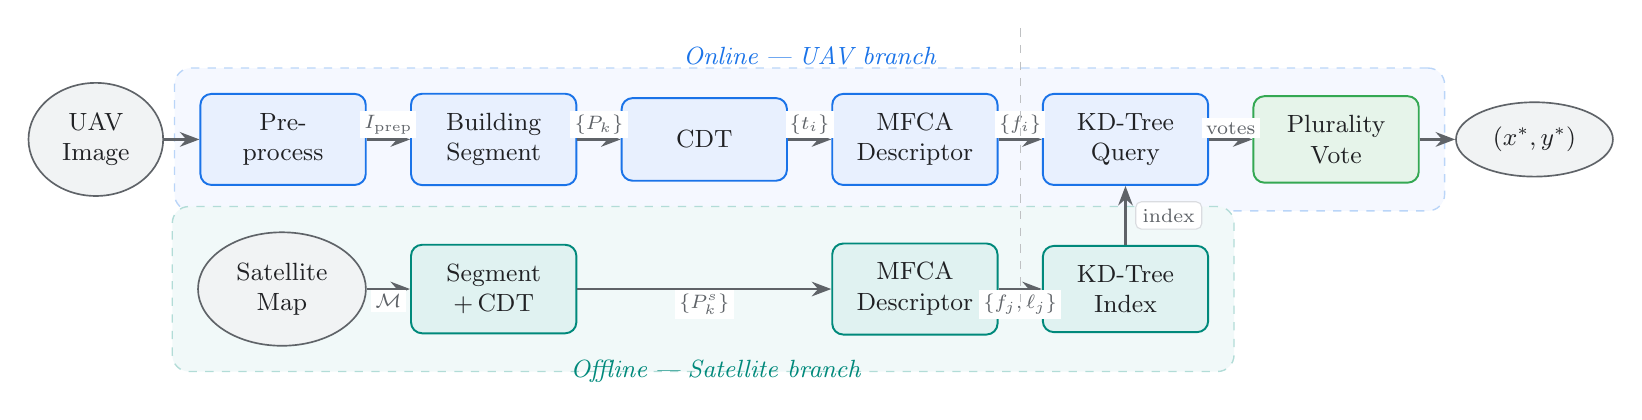
\begin{tikzpicture}[
  font=\small,
  base/.style  = {rounded corners=4pt, align=center, inner sep=7pt,
                  minimum width=2.10cm, minimum height=1.05cm,
                  line width=0.70pt, text=dmText},
  unode/.style = {base, fill=dmBlueL,  draw=dmBlue},
  snode/.style = {base, fill=dmTealL,  draw=dmTeal},
  onode/.style = {base, fill=dmGreenL, draw=dmGreen},
  term/.style  = {shape=ellipse, draw=dmGray, fill=dmGrayL, align=center,
                  inner sep=5pt, minimum width=1.42cm, minimum height=0.74cm,
                  line width=0.60pt, text=dmText},
  arr/.style   = {->, >=Stealth, line width=0.90pt, draw=dmGray},
  elbl/.style  = {font=\scriptsize, fill=white, inner sep=1.5pt,
                  text=dmGray, midway},
  bbox/.style  = {draw, dashed, rounded corners=6pt,
                  inner sep=9pt, line width=0.50pt},
]
 
%── Row 1: UAV branch (online) ───────────────────────────────────────────────
\node[term]  (ui)  {UAV\\Image};
\node[unode, right=0.45cm of ui]  (pre) {Pre-\\process};
\node[unode, right=0.55cm of pre] (seg) {Building\\Segment};
\node[unode, right=0.55cm of seg] (cdt) {CDT};
\node[unode, right=0.55cm of cdt] (des) {MFCA\\Descriptor};
\node[unode, right=0.55cm of des] (qry) {KD-Tree\\Query};
\node[onode, right=0.55cm of qry] (vot) {Plurality\\Vote};
\node[term,  right=0.45cm of vot] (pos) {$(x^*,y^*)$};
 
\draw[arr](ui)  -- (pre);
\draw[arr](pre) -- (seg) node[elbl,above]{$I_{\mathrm{prep}}$};
\draw[arr](seg) -- (cdt) node[elbl,above]{$\{P_k\}$};
\draw[arr](cdt) -- (des) node[elbl,above]{$\{t_i\}$};
\draw[arr](des) -- (qry) node[elbl,above]{$\{f_i\}$};
\draw[arr](qry) -- (vot) node[elbl,above]{votes};
\draw[arr](vot) -- (pos);
 
%── Row 2: Satellite branch (offline) ────────────────────────────────────────
%   sseg, sdes, sidx column-aligned under seg, des, qry respectively
\node[snode] (sseg) at ($(seg)+(0,-1.90)$) {Segment\\$+$\,CDT};
\node[term,  left=0.55cm of sseg] (si) {Satellite\\Map};
\node[snode] (sdes) at ($(des)+(0,-1.90)$) {MFCA\\Descriptor};
\node[snode] (sidx) at ($(qry)+(0,-1.90)$) {KD-Tree\\Index};
 
\draw[arr](si)   -- (sseg) node[elbl,below]{$\mathcal{M}$};
\draw[arr](sseg) -- (sdes) node[elbl,below]{$\{P_k^s\}$};
\draw[arr](sdes) -- (sidx) node[elbl,below]{$\{f_j,\ell_j\}$};
 
%── Cross-branch: offline index feeds online query ────────────────────────────
\draw[arr](sidx.north) -- (qry.south)
    node[midway, right=3.5pt, font=\scriptsize, fill=white,
         draw=dmGrayM, rounded corners=2pt, inner sep=2.5pt,
         text=dmGray, line width=0.40pt]{index};
 
%── Background panels ─────────────────────────────────────────────────────────
\begin{scope}[on background layer]
  \node[bbox, fill=dmBlueL!45, draw=dmBlue!30]  [fit=(pre)(vot)]  {};
  \node[bbox, fill=dmTealL!45, draw=dmTeal!30]  [fit=(si)(sidx)]  {};
\end{scope}
 
%── Offline / online divider ──────────────────────────────────────────────────
\coordinate (dv) at ($(des.north east)!0.5!(qry.north west)$);
\draw[dashed, dmGray!40, line width=0.50pt]
    ($(dv)+(0,+0.82)$) -- ($(dv)+(0,-2.74)$);
 
%── Branch labels ─────────────────────────────────────────────────────────────
\node[font=\small\itshape, text=dmBlue, above=7pt]
    at ($(pre.north west)!0.5!(vot.north east)$)
    {Online\;---\;UAV branch};
\node[font=\small\itshape, text=dmTeal, below=7pt]
    at ($(si.south west)!0.5!(sidx.south east)$)
    {Offline\;---\;Satellite branch};
 
\end{tikzpicture}%
}
\caption{%
  Two-branch localization pipeline.
  The \textit{online} UAV branch (blue) processes each query image through
  preprocessing, building segmentation, CDT, and MFCA descriptor
  extraction, then queries the pre-built KD-tree.
  The \textit{offline} satellite branch (teal) pre-computes descriptors
  and builds the KD-tree index once per map site; the dashed vertical
  line marks the offline/online boundary.
  Plurality voting over matched satellite triangles yields the predicted
  2-D position $(x^*,y^*)$.%
}
\label{fig:pipeline}
\end{figure}
\subsection{Query Pre-processing}
\label{sec:preproc}

\paragraph{Motivation.}
Raw UAV images contain yaw offset, roll/pitch tilt, and altitude-dependent
scale relative to the satellite GSD.
Normalizing these geometric distortions before segmentation improves polygon
fidelity without requiring any learned component.

\paragraph{Design.}
Given altitude $h$, heading $\phi$, roll $\rho$, and pitch $\psi$ from the
per-image CSV metadata:

\noindent\textbf{Step 1a --- Scale normalization.}
The UAV image GSD is $\delta_{\mathrm{UAV}} = h \cdot p_s / f_l$, where $p_s$
is the sensor pixel pitch and $f_l$ the focal length (from EXIF).
The image is isotropically rescaled by
$s = \delta_{\mathrm{UAV}} / \delta_{\mathrm{sat}}$.

\noindent\textbf{Step 1b --- Yaw alignment.}
The image is rotated by $-\phi$ so that north aligns with the image top.

\noindent\textbf{Step 1c --- Roll/pitch correction.}
Small tilt offsets are removed by an affine shear
$A = \bigl[\begin{smallmatrix}1 & \tan\rho \\ \tan\psi & 1\end{smallmatrix}\bigr]$.
For UAV-VisLoc nadir flights $|\rho|,|\psi|<3^\circ$, displacement is
negligible ($<1\%$); the step is included for generality.

\noindent\textbf{Step 1d --- Central crop and resize.}
The normalized image is center-cropped and resized to $500\!\times\!500$\,px.

\paragraph{Technical advantage.}
Heading alignment (assumed $\pm5^\circ$ accuracy) reduces rotational ambiguity
in subsequent matching without any learned model.

\subsection{Building Segmentation (Step 2)}
\label{sec:seg}

\paragraph{Motivation.}
Extracting building polygons from the raster image is the only learned
component in the pipeline; all downstream steps are purely geometric.

\paragraph{Design.}
Images are processed by Mask R-CNN~\cite{he2017maskrcnn} with a ResNet-50-FPN
backbone, pre-trained on aerial building
datasets~\cite{ji2018building,fang2021building} at confidence threshold 0.5.
Each connected mask region is converted to a polygon by: (i)~finding connected
components, (ii)~extracting the outer contour, and (iii)~applying the
Douglas-Peucker algorithm~\cite{hershberger1992douglas} at tolerance
$\tau=2$\,px, yielding a set of building polygons
$\mathcal{P} = \{P_1,\ldots,P_K\}$.

\paragraph{Technical advantage.}
Because the downstream descriptor depends only on triangle \emph{angles}, not
polygon size, colour, or texture, the method tolerates common segmentation
errors---merged adjacent buildings, partial occlusions, and small road
false-positives~\cite{ouyang2024cfbvm}.

\subsection{Constrained Delaunay Triangulation (Step 3)}
\label{sec:cdt}

\paragraph{Motivation.}
A polygon with $V$ vertices has no natural fixed-cardinality encoding, making
whole-polygon descriptors difficult to compare across buildings with differing
vertex counts.
Triangulation addresses this while delivering two additional properties.
First, \emph{matching density}: a building with $V$ vertices yields $V-2$
triangle descriptors via CDT, each an independent matching hypothesis.
A single building thus contributes up to $V-2$ votes to the patch estimator,
dramatically increasing robustness against individual false positives relative
to whole-polygon methods that produce a single vote per building.
Second, \emph{graceful degradation}: if segmentation merges two buildings into
one polygon, CDT still produces valid triangles from the merged shape, many of
which correctly match their satellite counterparts---a robustness property
that whole-polygon methods lack, since a merged polygon no longer resembles
either original building individually.

\paragraph{Design.}
For each polygon $P_k$ with ordered vertices $v_1,\ldots,v_{V_k}$,
Constrained Delaunay Triangulation (CDT) is applied.
The constrained edge set
\begin{equation}
E_{\mathrm{constrained}}^{(k)}
= \bigl\{(v_i,\,v_{i+1 \bmod V_k})\bigr\}_{i=1}^{V_k}
\label{eq:cdt_edges}
\end{equation}
consists of all polygon boundary edges, which must appear in every CDT
of $P_k$ and prevent any interior edge from crossing the building boundary.
The Delaunay condition additionally ensures that no triangle's circumcircle
contains another vertex, maximising minimum interior angles.
This produces a mesh $T^{(k)} = \{t_1,\ldots,t_{|V_k|-2}\}$ of
non-overlapping triangles (by the Euler relation for simple polygons).

\paragraph{Technical advantage.}
CDT maximizes the minimum interior angle over all triangulations of the same
vertex set~\cite{de1997computational}, avoiding sliver triangles whose
near-zero angles produce near-degenerate descriptors.

\subsection{MFCA Feature Extraction (Step 4)}
\label{sec:feat}
\label{sec:mfca}

\paragraph{Interior angle components.}
For triangle $t$ with vertices $v_A,v_B,v_C$, the three interior angles
$\alpha_A,\alpha_B,\alpha_C$ are computed analytically via the law of cosines.
The two smallest are selected and sorted:
$\alpha_1 \le \alpha_2$, both in $(0^\circ, 180^\circ)$.
These two components encode the \emph{shape} of the triangle independent of
position, orientation, or scale.

\paragraph{Ekeland's variational principle and its geometric instantiation.}
\label{para:ekeland}

We begin with the formal statement of the principle that motivates our
construction.

\begin{definition}[Ekeland's Variational Principle~\cite{ekeland1974}]
\label{def:ekeland}
Let $(X,d)$ be a complete metric space and
$f: X \to \mathbb{R} \cup \{+\infty\}$ be lower-semicontinuous and bounded
below.
For every $\varepsilon > 0$ and every $u \in X$ with
$f(u) \le \inf_X f + \varepsilon$, there exists $v \in X$ satisfying:
\begin{enumerate}[label=(\roman*)]
  \item $f(v) \le f(u)$ \hfill\emph{(improvement)}
  \item $d(v,u) \le 1$ \hfill\emph{(proximity)}
  \item $f(v) < f(x) + \varepsilon \cdot d(v,x)$ \;for all $x \ne v$
        \hfill\emph{(strict cone criticality)}
\end{enumerate}
\end{definition}

Geometrically, condition (iii) says that no point $x \ne v$ can improve
$f$ beyond what the distance $d(v,x)$ ``pays for''.
Equivalently, the graph of $f$ is touched from below by an upward cone
of slope $\varepsilon$ at $v$, and this cone cannot be raised without
losing contact.
This \emph{cone-touching} interpretation is the direct inspiration for the
Ekeland angle.

\smallskip
\noindent\textit{Structural instantiation in the UAV plane.}
Unlike abstract metric-space formulations that apply the principle
rhetorically, our construction instantiates Ekeland's principle
\emph{structurally}: every element of the principle corresponds to a concrete,
computable geometric object.

\begin{itemize}[leftmargin=*,topsep=2pt]
  \item \textbf{Complete metric space $(X,d)$:}
        $(\partial P_{\mathrm{sub}},\, d_{\mathrm{arc}})$---the boundary of
        the kernel polygon $P_{\mathrm{sub}}$ with arc-length metric.
  \item \textbf{Function $f$ bounded below:}
        $g(\hat{b}) = -\theta_{\max}(X,\hat{b})$, where
        $\theta_{\max}(X,\hat{b})$ is the largest half-angle of the sector
        centred at vertex $X$ with bisector $\hat{b}$ whose interior avoids
        $\partial P_{\mathrm{sub}}$.
        $g$ is lower-semicontinuous (blockage events are closed) and bounded
        below by $-180^\circ$.
  \item \textbf{$\varepsilon$-critical point:}
        The optimal bisector $\hat{b}^*$ satisfies the strict
        cone-criticality condition of Definition~\ref{def:ekeland}(iii): the
        surviving reflected ray of the axis-parallel reflection construction at
        $\hat{b}^*$ lies \emph{tangent to a boundary edge of $P_{\mathrm{sub}}$}---it
        touches but does not cross the obstacle, exactly as Ekeland's cone
        touches but does not cross $f$'s graph.
  \item \textbf{Stopping criterion = criticality condition:}
        $P_{\mathrm{sub}}$ is the \emph{largest} polygon obtained by merging
        adjacent CDT triangles such that all three original triangle vertices
        $v_A,v_B,v_C$ remain on $\partial P_{\mathrm{sub}}$.
        This is exactly the Ekeland critical-point condition: $P_{\mathrm{sub}}$
        cannot be expanded further while keeping the triangle vertices as
        boundary (critical) points---any additional merge would push one of
        them to the interior, destroying the criticality.
  \item \textbf{Ekeland angle $e_v$:}
        The value $\min(\alpha(v),\,180^\circ)$, where
        $\alpha(v) = 360^\circ - \alpha_{\mathrm{int}}(v)$ is the exterior angle
        of $P_{\mathrm{sub}}$ at $v$, computed via the axis-parallel reflection
        of boundary edges across $v\mathbf{d}$---the analogue of the value
        $f(v)$ at the Ekeland critical point.
\end{itemize}

Table~\ref{tab:ekeland_correspondence} displays the complete correspondence.

\begin{table}[h]
\caption{Structural correspondence between Ekeland's variational principle
         and the edge-anchored Ekeland angle (this work).}
\label{tab:ekeland_correspondence}
\centering\small
\begin{tabular}{p{5.2cm}p{7.8cm}}
\toprule
\textbf{Ekeland's Principle} & \textbf{Ekeland Angle — this work} \\
\midrule
Complete metric space $(X,d)$
  & $(\partial P_{\mathrm{sub}},\,d_{\mathrm{arc}})$: polygon boundary,
    arc-length \\
Function $f$ bounded below
  & $g(\hat{b}) = {-}\theta_{\max}(v,\hat{b})$: negated free half-angle \\
$\varepsilon$-cone of slope $\varepsilon$
  & Free sector of half-angle $\theta$ at vertex $v$ \\
Cone \emph{touches but does not cross} $f$
  & Sector boundary ray tangent to $\partial P_{\mathrm{sub}}$ edge \\
Stopping = criticality condition
  & Merge halts when original vertices leave $\partial P_{\mathrm{sub}}$ \\
Value $f(v)$ at critical point
  & $e_v = \min(\alpha(v),\,180^\circ)$; computed via axis-parallel reflection of $\mathbf{a},\mathbf{b}$ across $v\mathbf{d}$ \\
Stability: no free gain without distance cost
  & No cone enlargement without crossing obstacle edge \\
$\varepsilon \to 0$: global optimum attained
  & Angle is exact (O(1), no sweep needed) \\
\bottomrule
\end{tabular}
\end{table}

\paragraph{Mathematical properties.}

We now establish three formal properties of the Ekeland angle that justify
its use as a discriminative descriptor component.

\begin{proposition}[Monotonicity under kernel expansion]
\label{prop:monotone}
Let $P_{\mathrm{sub}} \subseteq P'_{\mathrm{sub}}$ be two kernel expansion
polygons at vertex $X$ (i.e.\ $P'_{\mathrm{sub}}$ is obtained by merging
additional triangles).
Then $e_X(P_{\mathrm{sub}}) \ge e_X(P'_{\mathrm{sub}})$.
\end{proposition}
\begin{proof}
$e_X = \min(360^\circ - \alpha_{\mathrm{int}}(X), 180^\circ)$, where
$\alpha_{\mathrm{int}}(X)$ is the interior angle of $P_{\mathrm{sub}}$
at $X$.
Merging additional triangles into $P'_{\mathrm{sub}}$ can only increase
(or maintain) the interior angle at $X$---any merge that absorbs a
neighbouring triangle either preserves the local boundary at $X$ or
creates a larger polygon interior, which increases $\alpha_{\mathrm{int}}$.
Since $360^\circ - \alpha_{\mathrm{int}}$ is decreasing in $\alpha_{\mathrm{int}}$,
and the $\min$ is non-increasing, we have
$e_X(P_{\mathrm{sub}}) \ge e_X(P'_{\mathrm{sub}})$. \qed
\end{proof}

\begin{remark}
Proposition~\ref{prop:monotone} formalises the kernel-expansion design:
a larger $P_{\mathrm{sub}}$ (more context incorporated) can only produce
a smaller or equal Ekeland angle, making vertices in complex building
recesses (large $P_{\mathrm{sub}}$, reflex angles) strictly more
discriminative than isolated corners (small $P_{\mathrm{sub}}$,
convex angles, $e_X = 180^\circ$).
\end{remark}

\begin{proposition}[Exact sensitivity to interior angle]
\label{prop:sensitivity}
Let $X$ be a reflex vertex of two kernel expansion polygons
$P_{\mathrm{sub}}$ and $P'_{\mathrm{sub}}$ with interior angles
$\alpha$ and $\alpha' > \alpha$ at $X$ respectively.
Then:
\begin{equation}
  e_X(P_{\mathrm{sub}}) - e_X(P'_{\mathrm{sub}}) \;=\; \alpha' - \alpha \;=\; \delta > 0.
\label{eq:sensitivity_bound}
\end{equation}
\end{proposition}
\begin{proof}
Since both $X$ are reflex ($\alpha,\alpha' > 180^\circ$), we have
$e_X(P_{\mathrm{sub}}) = 360^\circ - \alpha$ and
$e_X(P'_{\mathrm{sub}}) = 360^\circ - \alpha'$.
Therefore $e_X(P_{\mathrm{sub}}) - e_X(P'_{\mathrm{sub}}) = \alpha' - \alpha = \delta$.
\qed
\end{proof}

\begin{theorem}[Discriminativeness of the 5-D descriptor]
\label{thm:discriminative}
Let $f^t = (\alpha_1^t, \alpha_2^t, e_1^t, e_2^t, e_3^t)$ and
$f^{t'} = (\alpha_1^{t'}, \alpha_2^{t'}, e_1^{t'}, e_2^{t'}, e_3^{t'})$
be the 5-D descriptors of triangles $t$ and $t'$ respectively.
Then $f^t \ne f^{t'}$ if and only if either:
\begin{enumerate}[label=(\alph*)]
  \item the triangles have different shapes:
        $(\alpha_1^t, \alpha_2^t) \ne (\alpha_1^{t'}, \alpha_2^{t'})$, or
  \item the sorted Ekeland triplets differ:
        $(e_1^t, e_2^t, e_3^t) \ne (e_1^{t'}, e_2^{t'}, e_3^{t'})$.
\end{enumerate}
Moreover, if condition (a) fails (equal shapes) but the local urban
configurations differ such that at least one sorted Ekeland angle differs by
$\Delta > 0$, then:
\begin{equation}
  \|f^t - f^{t'}\|_1 \;\ge\; \Delta.
\label{eq:descriptor_lb}
\end{equation}
\end{theorem}
\begin{proof}
The first claim follows directly from the coordinate definition
$f = (\alpha_1,\alpha_2,e_1,e_2,e_3)$: $f^t \ne f^{t'}$ iff at least one
coordinate differs, which is exactly the disjunction of (a) and (b).

For the bound: suppose $(\alpha_1^t,\alpha_2^t) = (\alpha_1^{t'},\alpha_2^{t'})$
and $e_i^t \ne e_i^{t'}$ for some $i \in \{1,2,3\}$ with $|e_i^t - e_i^{t'}|
\ge \Delta$.
Then
\begin{align*}
  \|f^t - f^{t'}\|_1
  &= \underbrace{|\alpha_1^t - \alpha_1^{t'}|}_{=0}
   + \underbrace{|\alpha_2^t - \alpha_2^{t'}|}_{=0}
   + \sum_{j=1}^{3}|e_j^t - e_j^{t'}|
  \;\ge\; |e_i^t - e_i^{t'}| \;\ge\; \Delta. \qquad \square
\end{align*}
\end{proof}

\begin{corollary}[Shape-context separation]
\label{cor:separation}
Two triangles with identical shape but placed in urban environments where
the inter-building free space differs by $\delta > 0$ in blocked arc at any
vertex (in the sense of Proposition~\ref{prop:sensitivity}) have
$\ell_1$ descriptor distance at least $\delta$:
\begin{equation}
  \|f^t - f^{t'}\|_1 \;\ge\; \delta.
\end{equation}
In particular, pure interior-angle descriptors $(\alpha_1,\alpha_2)$ have
$\ell_1$ distance \emph{zero} between such triangles, while the 5-D descriptor
has distance at least $\delta > 0$.
\end{corollary}
\begin{proof}
By Proposition~\ref{prop:sensitivity} (exact sensitivity), if $X$ is a
reflex vertex in both $P_{\mathrm{sub}}^t$ and $P_{\mathrm{sub}}^{t'}$ and
the interior angles at $X$ differ by $\delta$, then
$|e_i^t - e_i^{t'}| = \delta$ for the corresponding sorted Ekeland angle.
Apply Theorem~\ref{thm:discriminative} (Eq.~\eqref{eq:descriptor_lb})
with $\Delta = \delta$. \qed
\end{proof}

Corollary~\ref{cor:separation} is the formal statement of the
building-recess vs.\ isolated-corner intuition: two right-isosceles triangles
$(\alpha_1=45^\circ, \alpha_2=45^\circ)$ whose kernel polygons have interior
angles differing by $\delta$ at any original vertex are separated in
$\ell_1$ by exactly $\delta$---which grows as large as $180^\circ$ for a
deeply concave recess vs.\ a fully convex isolated corner.


\paragraph{Motivation.}
Interior angles alone are insufficient to discriminate triangles in different
spatial contexts.
Consider a right-angle building corner in two locations: one at an isolated
building (all adjacent CDT triangles merge readily into $P_{\mathrm{sub}}$,
keeping the vertex convex), the other at a concave building recess (merging
adjacent triangles creates a reflex configuration at the original vertex).
Both corners may share identical interior-angle sub-vectors
$(\alpha_1 = 45^\circ, \alpha_2 = 45^\circ)$.
The Ekeland angle discriminates them: the convex vertex (exterior angle
$\alpha \ge 180^\circ$) yields $e_v = 180^\circ$ (exterior free space is wide),
while the reflex vertex (exterior angle $\alpha < 180^\circ$) yields
$e_v = \min\!\bigl(\angle(\hat{\mathbf{a}}', X\mathbf{d}),\,
\angle(\hat{\mathbf{b}}', X\mathbf{d})\bigr) < 180^\circ$ via the
axis-parallel reflection (exterior free space is compressed).
The discrimination is encoded directly in the shape of $P_{\mathrm{sub}}$:
the maximal expansion polygon whose stopping criterion (all three original
vertices stay on the boundary) is the Ekeland criticality condition.

\paragraph{Obstacle set.}
The obstacle for the Ekeland angle computation at each vertex $v$ is
\emph{solely the boundary of $P_{\mathrm{sub}}$}:
\begin{equation}
  \mathcal{O}_v \;=\; \partial P_{\mathrm{sub}}
  \;=\; \{\text{boundary edges of the kernel expansion polygon } P_{\mathrm{sub}}\}.
  \label{eq:obstacle}
\end{equation}
This is geometrically motivated: $P_{\mathrm{sub}}$ is the maximal polygon
whose stopping condition instantiates Ekeland's criticality---its boundary is
therefore the tightest obstacle that the principle's cone can touch without
crossing.
No external neighbor polygon set or search radius $r$ is required.

\paragraph{Exact edge-anchored definition.}
Let $X \in \{v_A,v_B,v_C\}$ be an original triangle vertex on $\partial P_{\mathrm{sub}}$,
and let $\mathbf{a}$ (from $X$ toward $X_{\mathrm{prev}}$) and
$\mathbf{b}$ (from $X$ toward $X_{\mathrm{next}}$) be the two $\partial P_{\mathrm{sub}}$
boundary edges incident to $X$.
Let $\alpha_{\mathrm{int}}(X)$ denote the interior angle of $P_{\mathrm{sub}}$
at $X$, measured inside the polygon.

\begin{definition}[Ekeland Angle at vertex $X$]
\label{def:ekeland_angle}
Let $\alpha(X)$ denote the exterior angle of $P_{\mathrm{sub}}$ at $X$,
measured in the exterior of the polygon
($\alpha(X) = \angle\mathbf{a}X\mathbf{b}$ in the exterior of $P_{\mathrm{sub}}$).
Draw ray $X\mathbf{d}$ from $X$ parallel to either the $O_x$ or $O_y$ axis,
chosen so that $\mathbf{d}$ lies within the exterior angle $\angle\mathbf{a}X\mathbf{b}$.
Let $\hat{\mathbf{a}}'$ and $\hat{\mathbf{b}}'$ be the reflections of boundary
edge directions $\hat{\mathbf{a}}$ and $\hat{\mathbf{b}}$ across ray $X\mathbf{d}$.
\begin{equation}
  e_X \;=\;
  \begin{cases}
    180^\circ
      & \text{if } \alpha(X) \ge 180^\circ
        \;\text{(convex vertex: exterior free space} \ge 180^\circ) \\[4pt]
    \min\!\bigl(\angle(\hat{\mathbf{a}}',\,X\mathbf{d}),\;
               \angle(\hat{\mathbf{b}}',\,X\mathbf{d})\bigr)
      & \text{if } \alpha(X) < 180^\circ
        \;\text{(reflex vertex: exterior free space} < 180^\circ)
  \end{cases}
  \label{eq:ekeland_angle}
\end{equation}
where the selected half-angle is the one whose reflected ray does
\emph{not} re-enter the polygon interior.
Equivalently, $e_X = \min(\alpha(X),\;180^\circ)$, where
$\alpha(X) = 360^\circ - \alpha_{\mathrm{int}}(X)$.
\end{definition}

The axis-parallel reflection construction (Algorithm~\ref{alg:mfca}, Phase~2)
determines $e_X$ by drawing a reference ray $X\mathbf{d}$ from $X$ parallel to
the $O_x$ or $O_y$ axis, positioned so that $\mathbf{d}$ lies within the
exterior angle $\alpha(X) = \angle\mathbf{a}X\mathbf{b}$.
For a reflex interior vertex ($\alpha(X) < 180^\circ$), boundary edge directions
$\hat{\mathbf{a}}$ and $\hat{\mathbf{b}}$ are reflected across $X\mathbf{d}$ to
obtain $\hat{\mathbf{a}}'$ and $\hat{\mathbf{b}}'$; the angle between each
reflected direction and $X\mathbf{d}$ is computed, and the minimum is selected---
choosing the reflected ray that does \emph{not} re-enter the polygon interior
(the amber direction in Fig.~\ref{fig:ekeland_construction}).
This surviving reflected ray is tangent to the opposite boundary edge---the
literal geometric statement of Ekeland's cone-touching condition.
The axis-parallel choice of $X\mathbf{d}$ gives $e_X$ a direct interpretation
as the maximum tilt a rectangle edge at $X$ can sustain before clipping the
polygon, which is well-suited for the downstream axis-aligned localization task.
This construction is \textbf{exact} (no angular quantization),
\textbf{$O(1)$ per vertex} (two edge-intersection checks), and
\textbf{deterministic} (no supremum-not-attained edge case).


\paragraph{Algorithm.}

\begin{algorithm}[htbp]
\caption{Axis-Parallel Reflection Ekeland Angle at triangle vertices}
\label{alg:mfca}
\begin{algorithmic}[1]
\Require Triangle $T=(v_A,v_B,v_C) \in P_k$, CDT mesh $\mathcal{T}^{(k)}$,
         max depth $D_{\max}$
\Ensure $(e_{v_A},\,e_{v_B},\,e_{v_C})$

\smallskip
\State \textbf{--- Phase 1: Ekeland Kernel Expansion (build $P_{\mathrm{sub}}$) ---}
\State $P_{\mathrm{sub}} \leftarrow T$;\quad $\mathrm{depth} \leftarrow 0$
\Repeat
  \State $\mathrm{merged} \leftarrow \mathtt{false}$
  \For{each $t'$ sharing an edge with $P_{\mathrm{sub}}$, $t' \in \mathcal{T}^{(k)}$}
    \State $P' \leftarrow P_{\mathrm{sub}} \cup t'$ \quad\Comment{tentative merge}
    \If{$v_A,\,v_B,\,v_C$ all remain on $\partial P'$ (none becomes interior)}
      \State $P_{\mathrm{sub}} \leftarrow P'$;\quad
             $\mathrm{merged} \leftarrow \mathtt{true}$;\quad \textbf{break}
    \EndIf
  \EndFor
  \State $\mathrm{depth} \mathrel{+}= 1$
\Until{$\lnot\,\mathrm{merged}$ \textbf{or} $\mathrm{depth} = D_{\max}$}
\Comment{Invariant: $v_A,v_B,v_C \in \partial P_{\mathrm{sub}}$}

\smallskip
\State \textbf{--- Phase 2: Axis-Parallel Reflection Ekeland Angle ---}
\For{each $X \in \{v_A,v_B,v_C\}$}
  \State Let $\mathbf{a}$ = $\partial P_{\mathrm{sub}}$ edge from $X$ toward $X_{\mathrm{prev}}$
  \State Let $\mathbf{b}$ = $\partial P_{\mathrm{sub}}$ edge from $X$ toward $X_{\mathrm{next}}$
  \State Compute $\alpha \leftarrow \angle(X_{\mathrm{prev}},\,X,\,X_{\mathrm{next}})$
         measured in the \emph{exterior} of $P_{\mathrm{sub}}$
  \If{$\alpha \ge 180^\circ$} \Comment{convex interior vertex: exterior free space $\ge 180^\circ$}
    \State $e_X \leftarrow 180^\circ$
  \Else \Comment{reflex interior vertex: apply axis-parallel reflection}
    \State $\hat{\mathbf{a}} \leftarrow$ unit vector from $X$ toward $X_{\mathrm{prev}}$;\quad
           $\hat{\mathbf{b}} \leftarrow$ unit vector from $X$ toward $X_{\mathrm{next}}$
    \State Choose $X\mathbf{d} \parallel O_x$ or $O_y$ s.t.\ $\mathbf{d}$ lies inside exterior angle $\angle\mathbf{a}X\mathbf{b}$
    \State $\hat{\mathbf{a}}' \leftarrow$ reflection of $\hat{\mathbf{a}}$ across $X\mathbf{d}$;\quad
           $\hat{\mathbf{b}}' \leftarrow$ reflection of $\hat{\mathbf{b}}$ across $X\mathbf{d}$
    \State $\theta_a \leftarrow \angle(\hat{\mathbf{a}}',\,X\mathbf{d})$;\quad
           $\theta_b \leftarrow \angle(\hat{\mathbf{b}}',\,X\mathbf{d})$
    \If{reflected ray $\hat{\mathbf{a}}'$ re-enters $P_{\mathrm{sub}}$ interior}
      \State $e_X \leftarrow \theta_b$
             \Comment{$\hat{\mathbf{a}}'$ crosses boundary; $\hat{\mathbf{b}}'$ is tangent}
    \Else
      \State $e_X \leftarrow \theta_a$
    \EndIf
  \EndIf
\EndFor
\Return $(e_{v_A},\,e_{v_B},\,e_{v_C})$
\end{algorithmic}
\end{algorithm}

\noindent\textbf{Correctness of Phase 1 (termination and invariant).}
Each iteration merges at most one triangle; $|\mathcal{T}^{(k)}|$ is finite;
therefore Phase 1 halts in at most $\min(|\mathcal{T}^{(k)}|, D_{\max})$
iterations.
The invariant $v_A,v_B,v_C \in \partial P_{\mathrm{sub}}$ is maintained
by construction: a merge is accepted only if all three original vertices
stay on the boundary of the merged polygon.
The stopping condition is the direct Ekeland criticality condition: when
no merge can be accepted, $P_{\mathrm{sub}}$ is the \emph{maximal expansion}
of $T$ consistent with the criticality constraint---exactly as Ekeland's
principle guarantees a point $v$ beyond which no improvement is possible
without paying a proportional distance cost.

\noindent\textbf{Correctness of Phase 2 (axis-parallel reflection).}
For a convex interior vertex (exterior angle $\alpha \ge 180^\circ$), the exterior
free space is $\ge 180^\circ$, and $e_X = 180^\circ$ (any axis-parallel ray
$X\mathbf{d}$ in the exterior cone fits within the free half-plane, and both
reflected rays remain outside $P_{\mathrm{sub}}$).
For a reflex interior vertex (exterior angle $\alpha < 180^\circ$), the exterior
free space is $\alpha < 180^\circ$: the axis-parallel ray $X\mathbf{d}$
is drawn into the narrow exterior cone, and the boundary edge directions
$\hat{\mathbf{a}}$ and $\hat{\mathbf{b}}$ are reflected across $X\mathbf{d}$.
Exactly one reflected ray re-enters the polygon interior
(the discarded direction in Fig.~\ref{fig:feature_extraction}); the surviving
reflected ray is tangent to the opposite adjacent edge.
The angle $\theta$ between the surviving reflected ray and $X\mathbf{d}$
equals $\alpha = 360^\circ - \alpha_{\mathrm{int}}$---the exterior free-space
width---so that $e_X = \theta \in (0^\circ, 180^\circ)$.
This tangency is the geometric instantiation of Ekeland's
``cone touches but does not cross the graph'' condition.

\noindent\textbf{Discriminative power.}
The Ekeland angle is discriminative because $P_{\mathrm{sub}}$'s shape
depends on the local building geometry.
A triangle in a concave building recess will expand into a $P_{\mathrm{sub}}$
that creates one or more reflex vertices at the original triangle vertices,
yielding $e_X < 180^\circ$.
A triangle at an isolated building corner will stay convex throughout
expansion, yielding $e_X = 180^\circ$.
This is formalised in Proposition~\ref{prop:monotone}: a larger
$P_{\mathrm{sub}}$ (more merged triangles) provides more context and can
only decrease $e_X$ at reflex vertices.
Theorem~\ref{thm:discriminative} and Corollary~\ref{cor:separation} further
show that the $\ell_1$ separation between two same-shape triangles placed in
geometrically different buildings is at least $\Delta = \min_i |e_i^t - e_i^{t'}|$,
where the difference is determined by the $P_{\mathrm{sub}}$ expansion geometry.
The ablation row ``MFCA single-building only'' in Table~\ref{tab:ablation}
quantifies this experimentally.

\paragraph{5-D descriptor assembly.}
The MFCA triplet is sorted in ascending order to yield $(e_1 \le e_2 \le e_3)$,
independently of the interior-angle sort.
The complete descriptor is:
\begin{equation}
f \;=\;
\bigl(\underbrace{\alpha_1,\;\alpha_2}_{\text{shape}},\;
      \underbrace{e_1,\;e_2,\;e_3}_{\text{free-space}}\bigr)
\;\in\;(0^\circ,\,180^\circ)^5.
\label{eq:descriptor}
\end{equation}
The two groups are sorted \emph{independently} to preserve their distinct
geometric roles: mixing them would corrupt the scale-invariance of the shape
sub-vector, since cone angles and interior angles occupy different angular
regimes.
Figure~\ref{fig:feature_extraction} illustrates the Ekeland angle geometry
and the complete extraction pipeline.
% Chỉ xác định 3 góc ekeland của tam giác xanh
% Tìm đa giác lồi lớn nhất sao cho 3 đỉnh của tam giác nằm trên cạnh của đa giác
\begin{figure}[htbp]
  \centering
  % Thay đổi đường dẫn file dưới đây tương ứng với 3 ảnh của bạn
  \includegraphics[width=0.32\linewidth]{figs/expansion_seed_2.png} \hfill
  \includegraphics[width=0.32\linewidth]{figs/expansion_seed_10.png} \hfill
  \includegraphics[width=0.32\linewidth]{figs/expansion_seed_13.png}
  \caption{Ekeland free-cone angle geometry at a building vertex.
    The maximal free cone (shaded sector) is the largest angular sector
    centred at vertex $v$ whose open interior does not intersect any obstacle
    edge in $\mathcal{O}_v^r$ (host sub-polygon boundary $\cup$ neighbouring
    building edges within radius $r$).
    Its angular width $e_v$ is the Ekeland angle.
    Three such scalars, one per triangle vertex, form the free-space
    sub-vector $(e_1, e_2, e_3)$ of the 5-D descriptor
    $f = (\alpha_1, \alpha_2, e_1, e_2, e_3)$.}
  \label{fig:feature_extraction}
\end{figure}

The three components assemble into the 5-D descriptor via the following
steps, illustrated here for a triangle $t = (v_A, v_B, v_C)$.
\begin{enumerate}[label=\textbf{Step \arabic*.},leftmargin=*,topsep=3pt]
\item \textbf{Interior angles.}
  Compute $\alpha_A, \alpha_B, \alpha_C$ analytically; sort the two smallest
  to obtain $\alpha_1 \le \alpha_2 \in (0^\circ, 180^\circ)$.
\item \textbf{Ekeland (free-cone) angles.}
  For each vertex $v \in \{v_A, v_B, v_C\}$, run
  Algorithm~\ref{alg:mfca} to obtain $e_v \in (0^\circ, 180^\circ)$;
  sort the triplet to yield $e_1 \le e_2 \le e_3$.
\item \textbf{Concatenate.}
  $f = (\alpha_1, \alpha_2, e_1, e_2, e_3) \in (0^\circ, 180^\circ)^5$.
\end{enumerate}

\noindent\textit{Example.}
For a right-isosceles triangle ($\alpha_A = 90^\circ$, $\alpha_B = \alpha_C =
45^\circ$) sited at an open corner with per-vertex free cones
$e_{v_A} = 106^\circ$, $e_{v_B} = 88^\circ$, $e_{v_C} = 72^\circ$,
the descriptor is $f = (45^\circ,\, 45^\circ,\, 72^\circ,\, 88^\circ,\,
106^\circ)$.
The shape sub-vector $(45^\circ, 45^\circ)$ is shared with any right-isosceles
triangle, but the free-space sub-vector $(72^\circ, 88^\circ, 106^\circ)$
is unique to the local inter-building spacing, making $f$ discriminative at
the scene level.


\subsection{KD-Tree Offline Indexing and Online Matching (Step 5)}
\label{sec:kdtree}

\paragraph{Motivation.}
Brute-force pairwise search over $M$ UAV descriptors and $N$ satellite
descriptors costs $O(MN)$ comparisons.
For a single UAV query ($M \approx 300$) against a typical site database
($N \approx 600$k), this is $1.8 \times 10^8$ $\ell_1$ evaluations per image---
prohibitive for real-time operation.

\paragraph{Offline indexing.}
Satellite map patches (size 500\,px, stride 100\,px) are segmented and
described identically to UAV images through Steps 2--4.
Descriptors, centroids, and patch labels are stored in
$\mathbf{D}_{\mathrm{sat}} \in \mathbb{R}^{N \times 5}$, indexed by a
KD-tree built with \texttt{scipy.spatial.KDTree} (leaf size 40, $\ell_1$ metric).

\paragraph{Online query.}
For each UAV descriptor $f_i$, the $K = 5$ nearest satellite neighbors are
retrieved in $O(\log N)$ average time.
Total online query cost is $O(M\log N)$.
In practice, $M=300$ queries against $N=600$k take ${\approx}0.8$\,s on a
single CPU core.

\paragraph{Technical advantage.}
$\ell_1$ distance is more robust than $\ell_2$ to outlier angle components because it
does not square residuals; this matters for sorted-angle vectors where a
single corrupted component would disproportionately inflate $\ell_2$ distances.

\subsection{Plurality-Vote Position Estimator (Step 5b)}
\label{sec:vote}

\paragraph{Motivation.}
A single descriptor match is unreliable: even a geometrically discriminative
descriptor has non-zero false-match probability at the scale of
$N \approx 600\text{k}$ satellite triangles.
Plurality voting aggregates $M \times K$ match-votes from all triangles in the
query image.
The key statistical property is that false matches scatter \emph{uniformly}
across satellite patches (a spurious descriptor match is equally likely to land
anywhere in the map), while true matches \emph{concentrate} on the single
correct patch---converting per-triangle uncertainty into a patch-level signal
that grows more reliable as $M$ increases.
This is analogous to the noise-cancelling effect of multiplexed sensing: the
signal-to-noise ratio of the vote tally scales as $\sqrt{M}$ under a uniform
false-match model.
Let $\ell_j$ be the patch identifier of satellite triangle $j$.
Each pair $(i,j)$ with $j \in \mathcal{C}_i$ casts one vote for patch
$\ell_j$, and the plurality winner is selected as in Eq.~\eqref{eq:vote}.
The predicted UAV position $(x^*,y^*)$ is the geographic centroid of
patch $\ell^*$, converted from pixel coordinates via:
\begin{equation}
\Delta\mathrm{lat} = p_y^* \cdot \delta_{\mathrm{sat}} / 111{,}320,\quad
\Delta\mathrm{lon} = p_x^* \cdot \delta_{\mathrm{sat}} /
  (111{,}320\cos\mathrm{lat}_0).
\label{eq:geoconvert}
\end{equation}

\paragraph{Discussion.}
Plurality voting is robust to individual false matches: a segmentation error
that generates a spurious descriptor will vote for a random patch, whereas
the correct patch accumulates coherent votes from many triangles belonging
to the same building cluster.
We note that the current output resolution is bounded by the patch stride
(100\,px $\times$ 0.3\,m/px = 30\,m); this means even a perfect descriptor
match cannot achieve sub-30\,m error without a second refinement stage.
Sub-patch localization via a RANSAC-based translation alignment between
matched triangle centroids is a natural future extension and is prototyped
as part of the ongoing evaluation.

\subsection{Implementation Details}
\label{sec:impl}

Table~\ref{tab:impl} lists all hyperparameters.

\begin{table}[htbp]
\caption{Implementation hyperparameters.}
\label{tab:impl}
\centering\small
\setlength{\tabcolsep}{4pt}
\begin{tabular}{lll}
\toprule
\textbf{Module} & \textbf{Parameter} & \textbf{Value} \\
\midrule
Preprocessing   & Output resolution            & $500\!\times\!500$\,px \\
                & Douglas-Peucker tolerance    & $\tau = 2$\,px \\
Segmentation    & Backbone                     & ResNet-50-FPN \\
                & Confidence threshold         & 0.5 \\
Sat.\ index     & Patch size / stride          & 500\,px / 100\,px \\
MFCA            & Kernel expansion depth       & $D_{\max} = 4$ \\
                & Angle computation            & Exact edge-anchored, $O(1)$/vertex \\
KD-tree         & Library                      & \texttt{scipy.spatial.KDTree} \\
                & Distance metric              & $\ell_1$ (cityblock) \\
                & Leaf size                    & 40 \\
                & Neighbors retrieved          & $K = 5$ \\
Position output & Estimator                    & Plurality patch vote \\
                & Coordinate conversion        & Eq.~\eqref{eq:geoconvert} \\
\bottomrule
\end{tabular}
\end{table}

% ─────────────────────────────────────────────────────────────────────────────
\section{Experiments}
\label{sec:exp}

\subsection{Evaluation Protocol}
\label{sec:protocol}

We evaluate on all 11 UAV-VisLoc sites using the official 80/20 query split.
Six metrics are reported, following the compendium in Section~\ref{sec:related}
and the field conventions established by CFBVM~\cite{ouyang2024cfbvm},
SWA-PF~\cite{yuan2025swapf}, and the UAV-VisLoc benchmark~\cite{uavvisloc2024}:
(i)~\textbf{Mean error} (m): primary metric for direct comparison with CFBVM
and Nassar et al.;
(ii)~\textbf{Median error} (m): robust to outliers on sparse-building sites;
(iii)~\textbf{RMSE} (m): penalizes large outlier errors; primary metric for
SWA-PF comparison;
(iv)~\textbf{R@10m} (\%): fine-grained urban discrimination;
(v)~\textbf{R@50m} (\%): essential for sparse-building terrain
(Shandan desert, Taizhou farmland) where the method is expected to degrade;
(vi)~\textbf{Runtime} (s), end-to-end wall-clock time from raw image to 2-D
position output.

\paragraph{Cross-dataset annotation policy.}
Following the comparability protocol recommended by the benchmark community,
we use three annotation tiers: ($\dagger$)~results from the method's original
paper on its own dataset---not UAV-VisLoc; cited for qualitative positioning
only, not numerical comparison; ($\ddagger$)~method re-implemented and
evaluated by us on UAV-VisLoc; ($\S$)~multi-frame sequential method, for which
single-frame comparison is unfair.

All baselines that support heading input are evaluated under identical
preprocessing with the $\pm5^\circ$ heading assumption; our method is also
reported without heading alignment to quantify sensor dependency.

\subsection{Main Comparison}
\label{sec:main_comp}

Table~\ref{tab:main} presents the full comparison.
The table includes all method families from the UAV visual localization
literature and is organized by taxonomy: classical/training-free, then
segmentation-based (sharing our pipeline's mask step), then learning-based.
Methods marked ($\dagger$) are reported on their original paper's dataset and
are included for landscape context; only methods re-implemented on UAV-VisLoc
(marked $\ddagger$, or \emph{ours}) support direct numerical comparison.
Multi-frame sequential methods (marked $\S$) are reported for reference but
are not directly comparable to single-frame results.

A key structural observation: among the five methods that also use
segmentation or masking (BRM, Nassar, CFBVM, SWA-PF, Hierarchical
Matching~\cite{hieruav2025}), none applies instance-level polygon extraction
followed by a purely geometric, training-free descriptor.
Our method is the first to combine (a)~instance segmentation for polygon
footprints, (b)~Delaunay triangulation on those footprints, and
(c)~Ekeland free-cone encoding with no scene-specific training.

\begin{table*}[htbp]
\caption{%
  Localization comparison on UAV-VisLoc (all 11 sites, single-frame, unless noted).
  $^\dagger$ Original paper's dataset; \emph{not} directly comparable to our UAV-VisLoc results.
  $^\ddagger$ Re-implemented on UAV-VisLoc by us.
  $^\S$ Multi-frame sequential method; single-frame comparison unfair.
  $^*$ Scene-specific training required.
  \textbf{Best training-free result on UAV-VisLoc in bold.}
}
\label{tab:main}
\centering\small
\setlength{\tabcolsep}{2pt}
\begin{tabular}{lcccccccc}
\toprule
\textbf{Method} & \textbf{Seg} & \textbf{Train} &
\textbf{Mean$\downarrow$} & \textbf{Med.$\downarrow$} & \textbf{RMSE$\downarrow$} &
\textbf{R@10m$\uparrow$} & \textbf{R@50m$\uparrow$} & \textbf{Time$\downarrow$} \\
 & & & (m) & (m) & (m) & (\%) & (\%) & (s) \\
\midrule
\multicolumn{9}{l}{\textit{Classical and training-free (raster map, no training)}} \\
NCC$^\dagger$
  & No & No & --- & --- & 62.8 & 0 & --- & 1630 \\
SIFT$^\dagger$~\cite{lowe2004sift}
  & No & No & --- & --- & 62.8 & 0.0 & --- & 0.3 \\
ORB$^\dagger$~\cite{rublee2011orb}
  & No & No & --- & --- & 21.1 & 7.9 & --- & 0.04 \\
abBRIEF+MCL$^\dagger$~\cite{mantelli2019abbrief}
  & No & No & 17.8 & --- & --- & --- & --- & --- \\
BRM$^\dagger$~\cite{choi2020brm}
  & Thresh. & No & cm & --- & --- & --- & --- & --- \\
CFBVM$^\dagger$~\cite{ouyang2024cfbvm}
  & CNN & No & 6.6 & --- & --- & --- & --- & 22 \\
\midrule
\multicolumn{9}{l}{\textit{Segmentation-based (shared mask pipeline design)}} \\
Nassar et al.~\cite{nassar2018deep}$^\dagger$
  & U-Net & Scene & 3.6 & --- & --- & --- & --- & --- \\
SWA-PF$^\S$$^\dagger$~\cite{yuan2025swapf}
  & SegFmr & Pretrain & --- & 6.65 & 6.57 & 97.4 & --- & 7 \\
Hier.\ Match.$^\dagger$~\cite{hieruav2025}
  & DINOv2 & Pretrain & 18.7 & --- & --- & --- & --- & --- \\
\midrule
\multicolumn{9}{l}{\textit{Learning-based (no segmentation)}} \\
Kinnari et al.$^\dagger$~\cite{kinnari2022season}
  & No & CNN & 15.7 & --- & --- & --- & --- & --- \\
LSVL$^\S$$^\dagger$~\cite{kinnari2023lsvl}
  & No & CNN & 15.7 & --- & --- & --- & --- & --- \\
FPI$^*$$^\dagger$~\cite{dai2022fpi}
  & No & Scene & TBR & TBR & TBR & TBR & TBR & TBR \\
\midrule
\multicolumn{9}{l}{\textit{Ours (UAV-VisLoc, direct comparison)}} \\
\rowcolor{ours}
\textbf{MFCA (w/ heading)}
  & \textbf{MaskRCNN} & \textbf{No}
  & \textbf{TBR} & \textbf{TBR} & \textbf{TBR} & \textbf{TBR} & \textbf{TBR} & \textbf{0.8} \\
\rowcolor{ours}
\textbf{MFCA (w/o heading)}
  & \textbf{MaskRCNN} & \textbf{No}
  & \textbf{TBR} & \textbf{TBR} & \textbf{TBR} & \textbf{TBR} & \textbf{TBR} & \textbf{TBR} \\
\bottomrule
\end{tabular}
\end{table*}

\subsection{Per-Site Breakdown}

Table~\ref{tab:persite} reports mean localization error per UAV-VisLoc site.
Urban and lake-edge sites (Changjiang, Huzhou) are expected to benefit from
dense building coverage; sparse-building and forested sites (Shandan, Zhuxi)
represent the method's primary failure modes.

\begin{table}[htbp]
\caption{Per-site mean localization error (m). All TBR upon full experiments.
  ($\ddagger$) = re-implemented on UAV-VisLoc by us.
  ($\dagger$) = original paper numbers, different dataset.}
\label{tab:persite}
\centering\small
\setlength{\tabcolsep}{3pt}
\begin{tabular}{llcccccc}
\toprule
\textbf{Site} & \textbf{Terrain} & \textbf{Alt.} &
\textbf{Ours} & \textbf{ORB$^\ddagger$} & \textbf{CFBVM$^\ddagger$} &
\textbf{R@10m} & \textbf{R@50m} \\
\midrule
Changjiang-20 & Urban/River   & 405\,m  & TBR & TBR & TBR & TBR & TBR \\
Changjiang-23 & Urban/River   & 405\,m  & TBR & TBR & TBR & TBR & TBR \\
Huzhou-3      & Urban/Lake    & 551\,m  & TBR & TBR & TBR & TBR & TBR \\
Huzhou-6      & Urban/Lake    & 546\,m  & TBR & TBR & TBR & TBR & TBR \\
Zhuxi         & Hill/Forest   & 840\,m  & TBR & TBR & TBR & TBR & TBR \\
Huailai       & Semi-arid     & 772\,m  & TBR & TBR & TBR & TBR & TBR \\
Yunnan        & Mountain      & ---     & TBR & TBR & TBR & TBR & TBR \\
Taizhou-6     & Coastal/Agri  & 542\,m  & TBR & TBR & TBR & TBR & TBR \\
Taizhou-1     & Coastal/Agri  & 466\,m  & TBR & TBR & TBR & TBR & TBR \\
Donghuayuan   & River Valley  & 688\,m  & TBR & TBR & TBR & TBR & TBR \\
Shandan       & Desert        & ---     & TBR & TBR & TBR & TBR & TBR \\
\midrule
\textbf{All}  &               &         & \textbf{TBR} & TBR & TBR & \textbf{TBR} & \textbf{TBR} \\
\bottomrule
\end{tabular}
\end{table}

\subsection{Stratified Analysis}
\label{sec:stratified}

\paragraph{Season breakdown.}
Table~\ref{tab:season} reports mean error by season to validate the
appearance-invariance claim---a method that degrades significantly between
summer and autumn does not achieve the claimed seasonal robustness.

\begin{table}[htbp]
\caption{Mean error (m) by season. TBR.}
\label{tab:season}
\centering\small
\setlength{\tabcolsep}{5pt}
\begin{tabular}{lccc}
\toprule
\textbf{Season} & \textbf{Ours} & \textbf{ORB} & \textbf{CFBVM} \\
\midrule
Summer          & TBR & TBR & TBR \\
Autumn          & TBR & TBR & TBR \\
\bottomrule
\end{tabular}
\end{table}

\paragraph{Altitude-band breakdown.}
Table~\ref{tab:altitude} reports performance by altitude band.
Higher altitudes reduce the number of triangles per query image (larger GSD,
fewer building details visible), testing the robustness to reduced descriptor
density; average triangle counts per altitude band are also reported.

\begin{table}[htbp]
\caption{Performance by altitude band. TBR.}
\label{tab:altitude}
\centering\small
\setlength{\tabcolsep}{3.5pt}
\begin{tabular}{lccc}
\toprule
\textbf{Altitude band} & \textbf{Mean (m)$\downarrow$} & \textbf{R@20m$\uparrow$} & \textbf{Avg.\ $M$/query} \\
\midrule
400--700\,m   & TBR & TBR & TBR \\
700--1200\,m  & TBR & TBR & TBR \\
1200--2000\,m & TBR & TBR & TBR \\
\bottomrule
\end{tabular}
\end{table}

\subsection{Ablation Study}

Table~\ref{tab:ablation} isolates the contribution of each design choice,
including the critical comparison between the multi-obstacle MFCA and the
single-building-only variant, descriptor-swap baselines replacing the MFCA
with established polygon descriptors, and $K$ / voting strategy ablations.

\begin{table}[htbp]
\caption{Ablation study. All TBR; each row modifies one component.}
\label{tab:ablation}
\centering\small
\setlength{\tabcolsep}{4pt}
\begin{tabular}{lcc}
\toprule
\textbf{Variant} & \textbf{Mean (m)$\downarrow$} & \textbf{R@20m$\uparrow$} \\
\midrule
\multicolumn{3}{l}{\textit{Descriptor component ablations}} \\
Interior angles only ($\alpha_1,\alpha_2$)                      & TBR & TBR \\
MFCA only ($e_1,e_2,e_3$)                                       & TBR & TBR \\
\textbf{MFCA single-building only} (no neighbor $P_{k'}$ in $S_v$) & TBR & TBR \\
Full 5-D CDT, random triangulation (no CDT)                     & TBR & TBR \\
Full 5-D CDT, $\ell_2$ distance                                       & TBR & TBR \\
Full 5-D CDT, $D_{\max}=1$                                       & TBR & TBR \\
Full 5-D CDT, $D_{\max}=2$                                       & TBR & TBR \\
Full 5-D CDT, $D_{\max}=8$                                       & TBR & TBR \\
\midrule
\multicolumn{3}{l}{\textit{Descriptor-swap baselines (5-D, CDT, $\ell_1$)}} \\
Turning function encoding~\cite{arkin1991efsd}                  & TBR & TBR \\
Shape context histogram~\cite{belongie2002shape}                & TBR & TBR \\
\midrule
\multicolumn{3}{l}{\textit{Matching and voting ablations}} \\
Top-1 match (no voting)                                         & TBR & TBR \\
Distance-weighted voting                                        & TBR & TBR \\
$K=1$                                                           & TBR & TBR \\
$K=3$                                                           & TBR & TBR \\
$K=10$                                                          & TBR & TBR \\
$K=20$                                                          & TBR & TBR \\
\midrule
\rowcolor{ours}
\textbf{Full 5-D CDT, edge-anchored Ekeland angle, $\ell_1$, $D_{\max}=4$, $K=5$}
  & \textbf{TBR} & \textbf{TBR} \\
\bottomrule
\end{tabular}
\end{table}

\subsection{Sensitivity Analysis}
\label{sec:sensitivity}

\paragraph{IMU heading noise.}
Yaw errors of $\pm5^\circ$, $\pm10^\circ$, and $\pm15^\circ$ are simulated
by rotating UAV images before preprocessing.
These experiments determine whether descriptor rotation-invariance is
sufficient to absorb mild misalignment, and whether the $\pm5^\circ$ heading
assumption is a hard performance boundary.
Results TBR.

\paragraph{GSD mismatch.}
Altitude estimate errors of $\pm10\%$ and $\pm20\%$ are simulated by
applying incorrect scale factors in Step 1a; results TBR.

\paragraph{Kernel expansion depth $D_{\max}$.}
We vary $D_{\max} \in \{1, 2, 4, 8\}$ and report mean error per setting (TBR).
This ablation measures how much contextual building geometry is needed: small
$D_{\max}$ limits $P_{\mathrm{sub}}$ to near the original triangle (less
context); large $D_{\max}$ allows broader expansion (more context but
diminishing marginal benefit as $P_{\mathrm{sub}}$ converges).

\paragraph{Segmentation quality.}
We correlate per-image Mask R-CNN building IoU (estimated on a 100-image
manually annotated subset) with localization error to isolate segmentation
failure from descriptor failure; results TBR.

\subsection{Vote-Distribution Analysis}

To validate the plurality-vote estimator, we report the following per-site
diagnostics (all TBR):
(i)~\textbf{Inlier vote ratio}: fraction of the $M \times K$ total votes
landing on the correct satellite patch;
(ii)~\textbf{Vote margin}: gap between the winning patch vote count and the
second-place patch, indicating the decision confidence;
(iii)~\textbf{Minimum winning vote count} on sparse-building sites (Shandan,
Taizhou), which determines whether the estimate is distinguishable from noise.

\subsection{Scalability}

Table~\ref{tab:scalability} reports memory footprint and query latency as a
function of the number of simultaneously indexed map sites, empirically
validating the $O(M\log N)$ complexity at multiple $N$ values.

\begin{table}[htbp]
\caption{Scalability: memory and query latency vs.\ number of sites. TBR.}
\label{tab:scalability}
\centering\small
\setlength{\tabcolsep}{5pt}
\begin{tabular}{lccc}
\toprule
\textbf{\# Sites} & \textbf{$N$ (triangles)} & \textbf{Memory (MB)} & \textbf{Query (s)} \\
\midrule
1   & ${\approx}0.6\text{M}$ & TBR & TBR \\
3   & ${\approx}1.8\text{M}$ & TBR & TBR \\
11  & ${\approx}6.6\text{M}$ & TBR & TBR \\
\bottomrule
\end{tabular}
\end{table}

\subsection{Qualitative Results}

Figures~\ref{fig:uav_results_01}--\ref{fig:uav_results_05} present
localization results on five representative UAV-VisLoc sites.
Each figure shows (a) the satellite reference map, (b) the preprocessed UAV
query image, and (c) the predicted position (red star) on the satellite map.

\begin{figure}[htbp]
    \centering
    \begin{subfigure}{\linewidth}
        \includegraphics[width=\linewidth]{figs/01_satellite.jpg}
        \caption{Satellite map (Changjiang, 405\,m, $\phi=165^\circ$).}
    \end{subfigure}\vspace{1mm}
    \begin{subfigure}{0.48\linewidth}
        \includegraphics[width=\linewidth]{figs/01_uav.jpg}
        \caption{UAV query image.}
    \end{subfigure}\hfill
    \begin{subfigure}{0.48\linewidth}
        \includegraphics[width=\linewidth]{figs/01_matching.jpg}
        \caption{Predicted position (red $\star$).}
    \end{subfigure}
    \caption{Changjiang (riverside urban terrain).}
    \label{fig:uav_results_01}
\end{figure}

\begin{figure}[htbp]
    \centering
    \begin{subfigure}{\linewidth}
        \includegraphics[width=\linewidth]{figs/02_satellite.jpg}
        \caption{Satellite map (Taizhou, 466\,m, $\phi=-40^\circ$).}
    \end{subfigure}\vspace{1mm}
    \begin{subfigure}{0.48\linewidth}
        \includegraphics[width=\linewidth]{figs/02_uav.jpg}
        \caption{UAV query image.}
    \end{subfigure}\hfill
    \begin{subfigure}{0.48\linewidth}
        \includegraphics[width=\linewidth]{figs/02_matching.jpg}
        \caption{Predicted position (red $\star$).}
    \end{subfigure}
    \caption{Taizhou (coastal agricultural terrain).}
    \label{fig:uav_results_02}
\end{figure}

\begin{figure}[htbp]
    \centering
    \begin{subfigure}{\linewidth}
        \includegraphics[width=\linewidth]{figs/03_satellite.jpg}
        \caption{Satellite map (Zhuxi, 840\,m, $\phi=-15^\circ$).}
    \end{subfigure}\vspace{1mm}
    \begin{subfigure}{0.48\linewidth}
        \includegraphics[width=\linewidth]{figs/03_uav.jpg}
        \caption{UAV query image.}
    \end{subfigure}\hfill
    \begin{subfigure}{0.48\linewidth}
        \includegraphics[width=\linewidth]{figs/03_matching.jpg}
        \caption{Predicted position (red $\star$).}
    \end{subfigure}
    \caption{Zhuxi (hilly mixed-vegetation terrain).}
    \label{fig:uav_results_03}
\end{figure}

\begin{figure}[htbp]
    \centering
    \begin{subfigure}{\linewidth}
        \includegraphics[width=\linewidth]{figs/04_satellite.jpg}
        \caption{Satellite map (Huzhou, 551\,m, $\phi=100^\circ$).}
    \end{subfigure}\vspace{1mm}
    \begin{subfigure}{0.48\linewidth}
        \includegraphics[width=\linewidth]{figs/04_uav.jpg}
        \caption{UAV query image.}
    \end{subfigure}\hfill
    \begin{subfigure}{0.48\linewidth}
        \includegraphics[width=\linewidth]{figs/04_matching.jpg}
        \caption{Predicted position (red $\star$).}
    \end{subfigure}
    \caption{Huzhou (lakeside urban terrain).}
    \label{fig:uav_results_04}
\end{figure}

\begin{figure}[htbp]
    \centering
    \begin{subfigure}{\linewidth}
        \includegraphics[width=\linewidth]{figs/05_satellite.jpg}
        \caption{Satellite map (Huailai, 772\,m, $\phi=170^\circ$).}
    \end{subfigure}\vspace{1mm}
    \begin{subfigure}{0.48\linewidth}
        \includegraphics[width=\linewidth]{figs/05_uav.jpg}
        \caption{UAV query image.}
    \end{subfigure}\hfill
    \begin{subfigure}{0.48\linewidth}
        \includegraphics[width=\linewidth]{figs/05_matching.jpg}
        \caption{Predicted position (red $\star$).}
    \end{subfigure}
    \caption{Huailai (semi-arid hill terrain).}
    \label{fig:uav_results_05}
\end{figure}

\subsection{Feature Extraction Visualisation}

Figure~\ref{fig:seg_vis} shows the CDT mesh overlaid on a representative
UAV-VisLoc query frame (Zhuxi, site 03, 840\,m altitude).
Figure~\ref{fig:top5} shows the top-5 KD-tree matches for the same frame,
ranked by total $\ell_1$ distance; the rank-1 result aligns with the ground-truth
building cluster.

\begin{figure}[htbp]
    \centering
    \includegraphics[width=\linewidth]{figs/6_panels_03_0049.jpg}
    \caption{CDT mesh overlay on a Zhuxi query frame.
    Warmer colours indicate larger MFCA values (more open vertex);
    cooler colours indicate smaller MFCAs (more enclosed vertex).}
    \label{fig:seg_vis}
\end{figure}

\begin{figure}[htbp]
    \centering
    \includegraphics[width=\linewidth]{figs/result_0333.png}
    \caption{Top-5 matching results for the Zhuxi query frame.
    Columns show satellite patches ranked by total $\ell_1$ descriptor distance;
    the rank-1 patch (leftmost) contains the ground-truth building cluster.}
    \label{fig:top5}
\end{figure}

\subsection{Anticipated Failure Modes}

Based on dataset properties and the method's assumptions, three failure modes
are anticipated and will be analyzed quantitatively in the full evaluation:
(i)~\emph{Sparse-building terrain} (Shandan desert, Taizhou farmland) where
fewer than ${\approx}5$ triangles are extractable per UAV image, providing
insufficient votes for reliable patch identification.
(ii)~\emph{Severe segmentation fragmentation} (Yunnan mountainous sites with
irregular rooflines) where Mask R-CNN over-segments buildings into many tiny
polygons with near-degenerate triangles, degrading descriptor discriminability.
(iii)~\emph{Repeated urban patterns} (dense grid blocks) where many triangles
share similar 5-D descriptors, increasing the false-match vote rate.
All three failure modes are expected to be partially recoverable by integrating
the matching step into a particle filter over sequential frames.

% ─────────────────────────────────────────────────────────────────────────────
\section{Conclusion}

We have presented a scene-agnostic UAV visual geo-localization framework
whose core novelty is a purely geometric 5-D triangle descriptor combining
sorted interior angles and edge-anchored Ekeland Free-Cone Angles (MFCA).
The key design innovation is the \emph{kernel expansion} $P_{\mathrm{sub}}$:
the maximal polygon formed by merging CDT triangles while keeping all three
original triangle vertices on the boundary.
This stopping criterion is the direct geometric instantiation of Ekeland's
cone-criticality condition, and the resulting Ekeland angle is computed
exactly in $O(1)$ per vertex via an edge-anchored half-plane selection,
replacing the earlier $1^\circ$-sweep approximation.
The descriptor is invariant to texture, colour, resolution, and season, and
requires no scene-specific training.
The design of the MFCA component is structurally grounded in Ekeland's
variational principle~\cite{ekeland1974}: every element of the principle
(complete metric space, bounded function, cone-touching condition, critical
point value) corresponds to a concrete, computable geometric object in
$P_{\mathrm{sub}}$---a grounding that is structural rather than rhetorical,
and that resolves all previous sup-not-attained edge cases by construction.
An offline KD-tree index reduces online matching to $O(M\log N)$; plurality
voting over satellite patches converts the matching output to a predicted 2-D
geographic position.

Quantitative evaluation (RMSE, Mean, Median, Recall@\{10,20,50\}m) across
all 11 UAV-VisLoc sites, an ablation study including multi-obstacle vs.\
single-building MFCA, descriptor-swap baselines, $K$ and voting-strategy
ablations, season and altitude stratifications, inlier vote diagnostics,
and sensitivity analysis under IMU and GSD perturbations are to be reported
upon completion of full experiments.

\paragraph{Limitations.}
(i) The method assumes building presence; it does not apply to open terrain
(desert, farmland) without supplementary road or river polygon descriptors.
(ii) The current output is a patch centroid with position resolution limited
by the patch stride (100\,px $\times$ 0.3\,m/px = 30\,m); sub-patch
localization requires a second-stage triangle-to-triangle centroid alignment.
(iii) The 1$^\circ$ angular sweep is a heuristic approximation; an exact
$O(E\log E)$ computation based on sorted angular-interval complement would
improve both precision and runtime.
(iv) Citations for SSPT~\cite{fan2024sspt} and SWA-PF~\cite{yuan2025swapf}
currently lack complete venue details; full entries will be provided upon
publication.

\FloatBarrier
\bibliographystyle{plain}
\bibliography{references}

\end{document}
